
\subsection{\label{sec:Tutorial-3d-hex8-friction}Fault Friction Examples}

PyLith features discussed in this tutorial:
\begin{itemize}
\item Static fault friction
\item Slip-weakening fault friction
\item Rate-and-state fault friction
\item Nonlinear solver
\end{itemize}

\subsubsection{Overview}

This set of examples provides an introduction to using fault friction
in static and quasi-static problems with PyLith. Dynamic problems
with fault friction are discussed in Section \vref{sec:example:shearwave:quad4}.
The boundary conditions are all either static or quasi-static Dirichlet
conditions, and only elastic materials are used. In all the fault
friction examples we apply axial (x) displacements on both the positive
and negative x-faces to maintain a compressive normal tractions on
the fault. Otherwise, there would be no frictional resistance. Fault
friction generates nonlinear behavior, so we use the nonlinear solver.
All of the examples are contained in the directory \texttt{examples/3d/hex8},
and the corresponding \texttt{.cfg} files are \texttt{step10.cfg},
\texttt{step11.cfg}, \texttt{step12.cfg}, \texttt{step13.cfg}, and
\texttt{step14.cfg}. Each example may be run as follows:
\begin{lyxcode}
pylith~stepXX.cfg
\end{lyxcode}
This will cause PyLith to read the default parameters in \texttt{pylithapp.cfg},
and then override or augment them with the additional parameters in
the \texttt{stepXX.cfg} file. Each \texttt{.cfg} file is extensively
documented, to provide detailed information on the various parameters.


\subsubsection{Step10 - Static Friction (Stick) with Static Dirichlet Boundary Conditions}

The \texttt{step10.cfg} file defines a problem that is identical to
example step01, except for the presence of a vertical fault with static
friction. In this case, the applied displacements are insufficient
to cause the fault to slip, so the solution is identical to that in
example step01. As in previous examples involving faults, we must
first provide an array defining the fault interfaces:
\begin{lyxcode}
{[}pylithapp.timedependent{]}

\#~Set~interfaces~to~an~array~of~1~fault:~'fault'.

interfaces~=~{[}fault{]}
\end{lyxcode}
Since all fault friction models are nonlinear we must also use the
nonlinear solver:
\begin{lyxcode}
{[}pylithapp.timedependent.implicit{]}

\#~Fault~friction~is~a~nonlinear~problem~so~we~need~to~use~the~nonlinear

\#~solver.

solver~=~pylith.problems.SolverNonlinear
\end{lyxcode}
We need to change the fault interface from the default (\texttt{FaultCohesiveKin})
to \texttt{FaultCohesiveDyn} and we set the friction model to use:
\begin{lyxcode}
{[}pylithapp.timedependent.interfaces{]}

\#~Change~fault~to~dynamic~fault~interface.

fault~=~pylith.faults.FaultCohesiveDyn~\\
~\\


{[}pylithapp.timedependent.interfaces.fault{]}

\#~Use~the~static~friction~model.

friction~=~pylith.friction.StaticFriction
\end{lyxcode}
The \texttt{StaticFriction} model requires values for the coefficient
of friction and the cohesion (see Section \vref{sec:fault:constitutive:models}).
We provide both of these using a \texttt{UniformDB}:
\begin{lyxcode}
{[}pylithapp.timedependent.interfaces.fault{]}

\#~Set~static~friction~model~parameters~using~a~uniform~DB.~Set~the

\#~static~coefficient~of~friction~to~0.6~and~cohesion~to~0.0~Pa.

friction.db\_properties~=~spatialdata.spatialdb.UniformDB

friction.db\_properties.label~=~Static~friction

friction.db\_properties.values~=~{[}friction-coefficient,cohesion{]}

friction.db\_properties.data~=~{[}0.6,0.0{*}Pa{]}
\end{lyxcode}
Fault friction models require additional PETSc settings:
\begin{lyxcode}
\#~NOTE:~There~are~additional~settings~specific~to~fault~friction.

{[}pylithapp.petsc{]}

\#~Friction~sensitivity~solve~used~to~compute~the~increment~in~slip

\#~associated~with~changes~in~the~Lagrange~multiplier~imposed~by~the

\#~fault~constitutive~model.

friction\_pc\_type~=~asm

friction\_sub\_pc\_factor\_shift\_type~=~nonzero

friction\_ksp\_max\_it~=~25

friction\_ksp\_gmres\_restart~=~30

\#~Uncomment~to~view~details~of~friction~sensitivity~solve.

\#friction\_ksp\_monitor~=~true

\#friction\_ksp\_view~=~true

friction\_ksp\_converged\_reason~=~true


\end{lyxcode}
When we have run the simulation, the output VTK files will be contained
in \texttt{examples/3d/hex8/output} (all with a pvrefix of \texttt{step10}).
Results using ParaView are shown in Figure \vref{fig:step10-fault-traction-slip}.

\begin{figure}
\begin{centering}
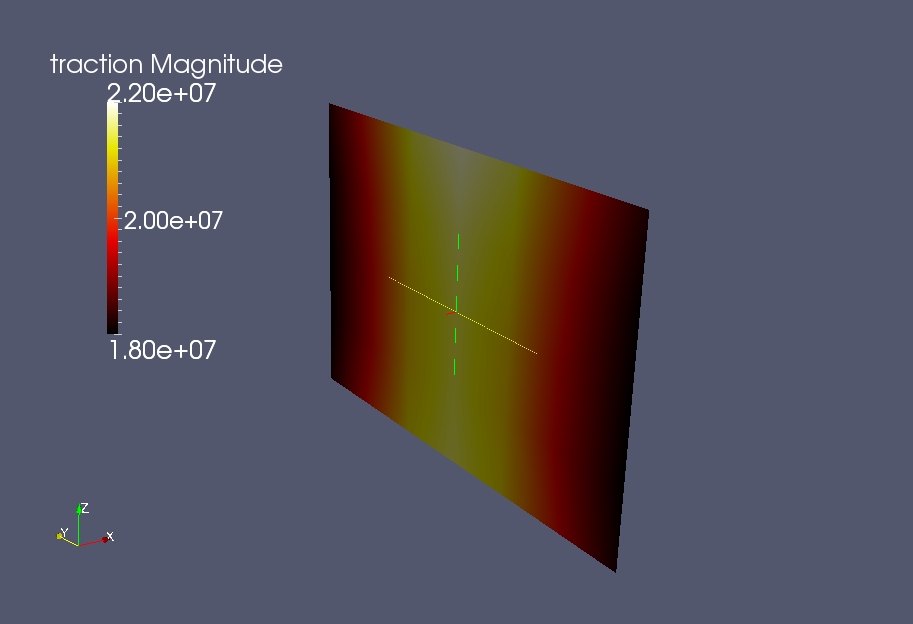
\includegraphics[width=10cm]{tutorials/3dhex8/figs/step10-fault-traction-slip}
\par\end{centering}

\caption{Magnitude of tractions on the fault for example step10 visualized
using ParaView. \label{fig:step10-fault-traction-slip}}
\end{figure}



\subsubsection{Step11 - Static Friction (Slip) with Static Dirichlet Boundary Conditions}

In step11 we apply twice as much shear displacement as in step10,
which is sufficient to induce slip on the fault. All other settings
are identical. To change the amount of shear displacement, we change
the spatial database for the positive and negative x-faces to a \texttt{UniformDB},
and apply the altered values within the \texttt{.cfg} file:
\begin{lyxcode}
\#~+x~face

{[}pylithapp.timedependent.bc.x\_pos{]}

bc\_dof~=~{[}0,~1{]}

label~=~face\_xpos

db\_initial~=~spatialdata.spatialdb.UniformDB

db\_initial.label~=~Dirichlet~BC~on~+x

db\_initial.values~=~{[}displacement-x,displacement-y{]}

db\_initial.data~=~{[}-1.0{*}m,2.0{*}m{]}



\#~-x~face

{[}pylithapp.timedependent.bc.x\_neg{]}

bc\_dof~=~{[}0,~1{]}

label~=~face\_xneg

db\_initial~=~spatialdata.spatialdb.UniformDB

db\_initial.label~=~Dirichlet~BC~on~-x

db\_initial.values~=~{[}displacement-x,displacement-y{]}

db\_initial.data~=~{[}1.0{*}m,-2.0{*}m{]}
\end{lyxcode}
When we have run the simulation, the output VTK files will be contained
in \texttt{examples/3d/hex8/output} (all with a pvrefix of \texttt{step11}).
Results using ParaView are shown in Figure \vref{fig:step11-fault-traction-slip}.

\begin{figure}
\begin{centering}
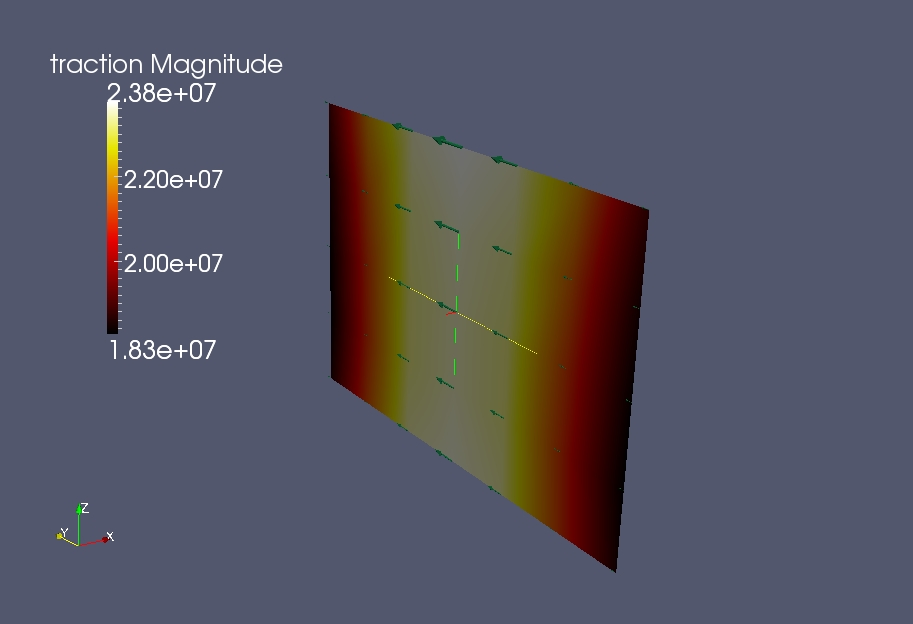
\includegraphics[width=10cm]{tutorials/3dhex8/figs/step11-fault-traction-slip}
\par\end{centering}

\caption{Magnitude of tractions on the fault for example step10 visualized
using ParaView. Vectors of fault slip are also plotted. Note that
PyLith outputs slip in the fault coordinate system, so we transform
them to the global coordinate system using the Calculator in ParaView.
A more general approach involves outputing the fault coordinate system
information and using these fields in the Calculator. \label{fig:step11-fault-traction-slip}}
\end{figure}



\subsubsection{Step12 - Static Friction with Quasi-Static Dirichlet Boundary Conditions}

The \texttt{step12.cfg} file describes a problem that is similar to
examples step10 and step11, except that we apply velocity boundary
conditions and run the simulation for 200 years. Once fault friction
is overcome, the fault slips at a steady rate. To prevent convergence
problems we set the time step size to a constant value of 5 years:
\begin{lyxcode}
\#~Change~the~total~simulation~time~to~200~years,~and~use~a~constant~time

\#~step~size~of~5~years.

{[}pylithapp.timedependent.implicit.time\_step{]}

total\_time~=~200.0{*}year

dt~=~5.0{*}year
\end{lyxcode}
As in the other fault friction examples, we apply initial displacements
along the x-axis (to maintain a compressive stress on the fault),
and we apply velocity boundary conditions that yield a left-lateral
sense of motion:
\begin{lyxcode}
\#~+x~face~-{}-~Dirichlet

{[}pylithapp.timedependent.bc.x\_pos{]}

bc\_dof~=~{[}0,1{]}

label~=~face\_xpos

db\_initial~=~spatialdata.spatialdb.UniformDB

db\_initial.label~=~Dirichlet~BC~on~+x

db\_initial.values~=~{[}displacement-x,displacement-y{]}

db\_initial.data~=~{[}-1.0{*}m,0.0{*}m{]}

db\_rate~=~spatialdata.spatialdb.UniformDB

db\_rate.label~=~Dirichlet~rate~BC~on~+x

db\_rate.values~=~{[}displacement-rate-x,displacement-rate-y,rate-start-time{]}

db\_rate.data~=~{[}0.0{*}cm/year,1.0{*}cm/year,0.0{*}year{]}~\\
~\\


\#~-x~face

{[}pylithapp.timedependent.bc.x\_neg{]}

bc\_dof~=~{[}0,~1{]}

label~=~face\_xneg

db\_initial.label~=~Dirichlet~BC~on~-x

db\_rate~=~spatialdata.spatialdb.UniformDB

db\_rate.label~=~Dirichlet~rate~BC~on~-x

db\_rate.values~=~{[}displacement-rate-x,displacement-rate-y,rate-start-time{]}

db\_rate.data~=~{[}0.0{*}cm/year,-1.0{*}cm/year,0.0{*}year{]}
\end{lyxcode}
For this example, we keep the same coefficient of friction as examples
step10 and step11, but we include a cohesion of 2 MPa:
\begin{lyxcode}
{[}pylithapp.timedependent.interfaces.fault{]}

\#~Set~static~friction~model~parameters~using~a~uniform~DB.~Set~the

\#~static~coefficient~of~friction~to~0.6~and~cohesion~to~2.0~MPa.

friction.db\_properties~=~spatialdata.spatialdb.UniformDB

friction.db\_properties.label~=~Static~friction

friction.db\_properties.values~=~{[}friction-coefficient,cohesion{]}

friction.db\_properties.data~=~{[}0.6,2.0{*}MPa{]}
\end{lyxcode}
When we have run the simulation, the output VTK files will be contained
in \texttt{examples/3d/hex8/output} (all with a pvrefix of \texttt{step12}).
Results using ParaView are shown in Figure \vref{fig:step12-displ-t200}.

\begin{figure}
\begin{centering}
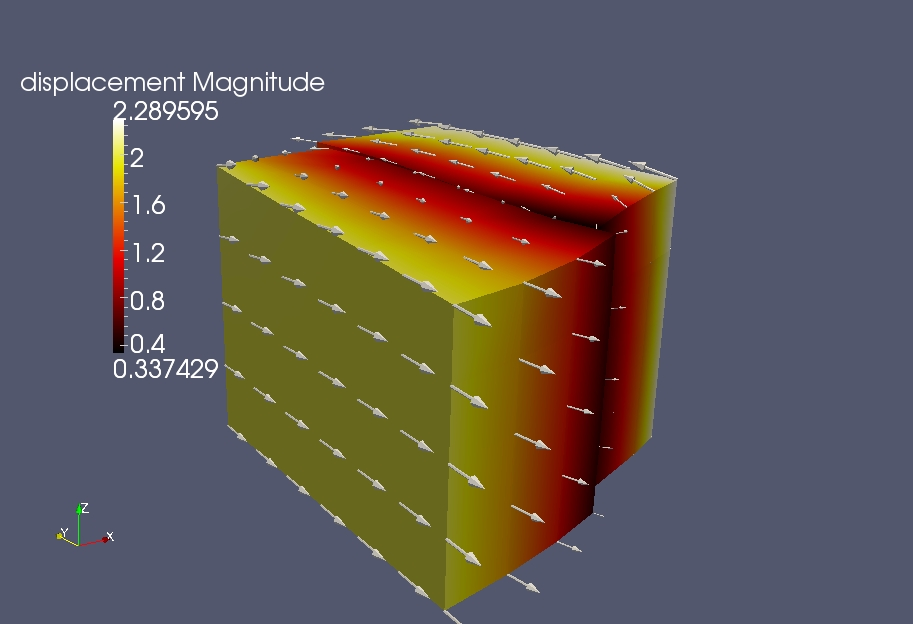
\includegraphics[width=10cm]{tutorials/3dhex8/figs/step12-displ-t200}
\par\end{centering}

\caption{Displacement field for example step12 at t = 200 years visualized
using ParaView. The mesh has been distorted by the computed displacements
(magnified by 500), and the vectors show the computed displacements.\label{fig:step12-displ-t200}}
\end{figure}



\subsubsection{Step13 - Slip-Weakening Friction with Quasi-Static Dirichlet Boundary
Conditions}

In this example we replace the static friction fault constitutive
model in step12 with a slip-weakening friction fault constitutive
model. Fault friction is overcome at about t = 80 years, the fault
slips in each subsequent time step. We again use a constant time step
size of 5 years and apply the same intial displacement and velocity
boundary conditions.

We first define the friction model for the simulation:
\begin{lyxcode}
{[}pylithapp.timedependent.interfaces.fault{]}

\#~Use~the~slip-weakening~friction~model.

friction~=~pylith.friction.SlipWeakening
\end{lyxcode}
The slip-weakening constitutive model requires a static coefficient
of friction, a dynamic coefficient of friction, a slip weakening parameter,
and a cohesion (see Section \vref{sec:fault:constitutive:models}):
\begin{lyxcode}
{[}pylithapp.timedependent.interfaces.fault{]}

\#~Set~slip-weakening~friction~model~parameters~using~a~uniform~DB.~Set~the

\#~parameters~as~follows:

\#~static~coefficient~of~friction:~0.6

\#~dynamic~coefficient~of~friction:~0.5

\#~slip-weakening~parameter:~0.2~m

\#~cohesion:~0~Pa

friction.db\_properties~=~spatialdata.spatialdb.UniformDB

friction.db\_properties.label~=~Slip~weakening

friction.db\_properties.values~=~{[}static-coefficient,dynamic-coefficient,~\\
slip-weakening-parameter,cohesion{]}

friction.db\_properties.data~=~{[}0.6,0.5,0.2{*}m,0.0{*}Pa{]}
\end{lyxcode}
When we have run the simulation, the output VTK files will be contained
in \texttt{examples/3d/hex8/output} (all with a pvrefix of \texttt{step1}3).
Results using ParaView are shown in Figure \vref{fig:step13-displ-t200}.

\begin{figure}
\begin{centering}
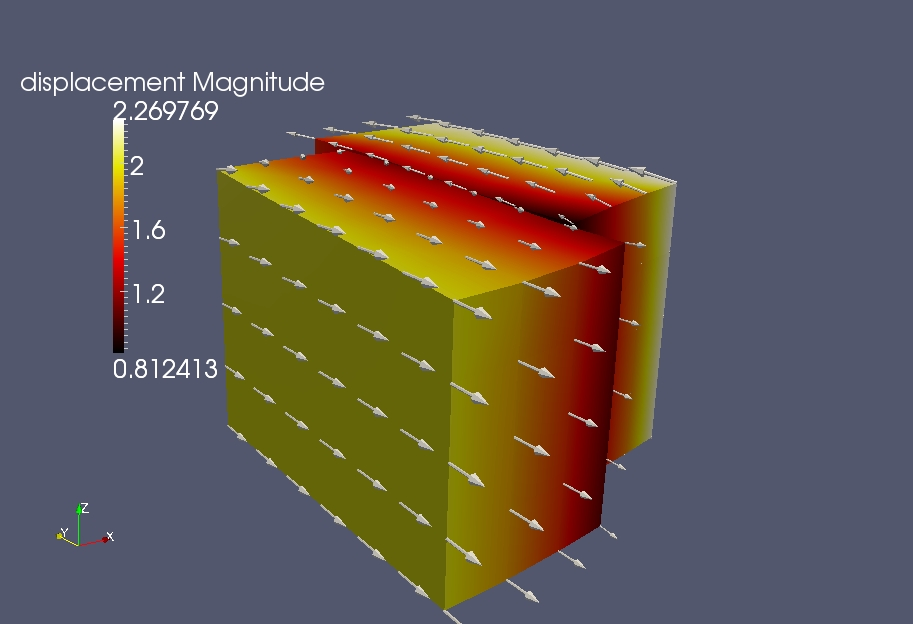
\includegraphics[width=10cm]{tutorials/3dhex8/figs/step13-displ-t200}
\par\end{centering}

\caption{Displacement field for example step13 at t = 200 years visualized
using ParaView. The mesh has been distorted by the computed displacements
(magnified by 500), and the vectors show the computed displacements.\label{fig:step13-displ-t200}}
\end{figure}



\subsubsection{Step14 - Rate-and-State Friction with Quasi-Static Dirichlet Boundary
Conditions}

In step14 we use a rate-and-state friction model with an ageing law
instead of a slip-weakening friction model. Slip begins to occur at
about t = 45 years, and continues in each subsequent time step. We
again use a constant time step size of 5 years and apply the same
intial displacement and velocity boundary conditions.

We first define the friction model for the simulation:
\begin{lyxcode}
{[}pylithapp.timedependent.interfaces.fault{]}

\#~Use~the~rate-and-state~aging~friction~model.

friction~=~pylith.friction.RateStateAgeing
\end{lyxcode}
The rate-and-state constitutive model requires a vreference coefficient
of friction, a vreference slip rate, a slip weakening parameter, an
a-value, a b-value, and a cohesion (see \vref{sec:fault:constitutive:models}):
\begin{lyxcode}
{\small{}{[}pylithapp.timedependent.interfaces.fault{]}}{\small \par}

{\small{}\#~Set~rate-and-state~parameters~using~a~UniformDB.~Set~the~parameters~as}{\small \par}

{\small{}\#~follows:}{\small \par}

{\small{}\#~vreference~coefficient~of~friction:~0.6}{\small \par}

{\small{}\#~vreference~slip~rate:~1.0e-06~m/s}{\small \par}

{\small{}\#~slip-weakening~parameter:~0.037~m}{\small \par}

{\small{}\#~a:~0.0125}{\small \par}

{\small{}\#~b:~0.0172}{\small \par}

{\small{}\#~cohesion:~0~Pa}{\small \par}

{\small{}friction.db\_properties~=~spatialdata.spatialdb.UniformDB}{\small \par}

{\small{}friction.db\_properties.label~=~Rate~State~Ageing}{\small \par}

{\small{}friction.db\_properties.values~=~{[}vreference-friction-coefficient,vreference-slip-rate,}~\\
{\small{}characteristic-slip-distance,constitutive-parameter-a,constitutive-parameter-b,cohesion{]}}{\small \par}

{\small{}friction.db\_properties.data~=~{[}0.6,1.0e-6{*}m/s,0.0370{*}m,0.0125,0.0172,0.0{*}Pa{]}}{\small \par}
\end{lyxcode}
For this model, we also want to set the initial value of the state
variable:
\begin{lyxcode}
{[}pylithapp.timedependent.interfaces.fault{]}

\#~Set~spatial~database~for~the~initial~value~of~the~state~variable.

friction.db\_initial\_state~=~spatialdata.spatialdb.UniformDB

friction.db\_initial\_state.label~=~Rate~State~Ageing~State

friction.db\_initial\_state.values~=~{[}state-variable{]}

friction.db\_initial\_state.data~=~{[}92.7{*}s{]}
\end{lyxcode}
When we have run the simulation, the output VTK files will be contained
in \texttt{examples/3d/hex8/output} (all with a pvrefix of \texttt{step14}).
Results using ParaView are shown in Figure \vref{fig:step14-displ-t200}.

\begin{figure}
\begin{centering}
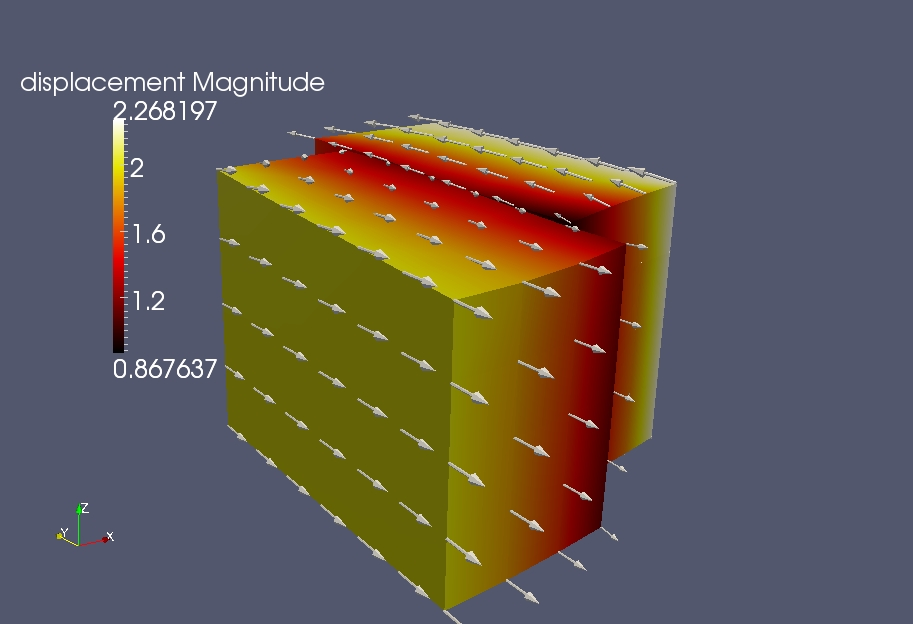
\includegraphics[width=10cm]{tutorials/3dhex8/figs/step14-displ-t200}
\par\end{centering}

\caption{Displacement field for example step14 at t = 200 years visualized
using ParaView. The mesh has been distorted by the computed displacements
(magnified by 500), and the vectors show the computed displacements.\label{fig:step14-displ-t200}}
\end{figure}

